\documentclass{scrartcl}
\usepackage[utf8]{inputenc}
\usepackage[T1]{fontenc}
\usepackage{lmodern}
\usepackage[ngerman]{babel}
\usepackage{amsmath}
\usepackage{amssymb}
\usepackage{stmaryrd}
\usepackage{blindtext}
\usepackage{graphicx}
\title{31. Beispiele fuer Gruppen}
\author{Adrian Hille}
\begin{document}
\Large 31. Beispiele f\"ur Gruppen\\
\\
\normalsize
Beispiele:\\
a) $(\mathbb{Z}, +, -, 0)$\\
+...Addition\\
-...$x \mapsto -x$\\
\\
b) $\mathbb{Z}_n = \{0,..., n-1\}$\\
$(\mathbb{Z}_n, +, -, 0)$\\
+/-...(modulo n)\\
\\
c) Die von 0 verschiedenen rationalen Zahlen bilden bzgl. der Multiplikation eine Gruppe.\\
\\
d) Sei $D= \{1, 2, 3\}$.  Die Menge aller Permutationen auf D bildet eine Gruppe bzgl. $\circ$ (Komposition von Funktion)\\
\\
e)\\
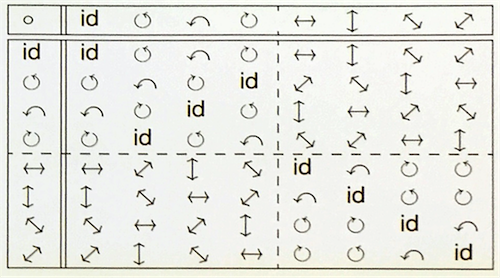
\includegraphics{Symmetrien.png}
\\
\\
\large Gruppen allgemein:
\normalsize
\begin{enumerate}
	\item $\circ$ ist assoziativ
	\item $\forall g \in G gibt es ein Element g^{-1}: g = g^{-1} = g^{-1} \circ g = e$ (Inverses Element)
	\item $\forall g \in G \quad g \circ e = e \circ g = g$ (e...neutrales Element)
\end{enumerate}

Beispiel:\\
$(\mathbb{Z}, +, -, 0) \qquad \forall g,h \in G \qquad g \circ h = h \circ g$ (abelsche Gruppe) ist kommutativ\\
$(\mathbb{Z}_n, +_{mod n}, -, 0)$\\
(Permutationen von $\{1, 2, 3\}, 0, \circ, ^{-1}, id$) $\to$ NICHT abelsch\\\\
$g := \binom{1 \quad 2 \quad 3}{2 \quad 3 \quad 1} \qquad h:= \binom{1 \quad 2 \quad 3}{2 \quad 1 \quad 3} $\\\\
$g \circ h = \binom{1 \quad 2 \quad 3}{3 \quad 2 \quad 1} \qquad h \circ g = \binom{1 \quad 2 \quad 3}{1 \quad 3 \quad 2}$\\\\

\end{document}